%%%%%%%%%%%%%%%%%%%%%%%%%%%%%%%%%%%%%%%%%%%%%%%%%%%%%%%%%%%%%%%%%%%%%%%%%%%%%%%
% Chapter: Background
%%%%%%%%%%%%%%%%%%%%%%%%%%%%%%%%%%%%%%%%%%%%%%%%%%%%%%%%%%%%%%%%%%%%%%%%%%%%%%%
\chapter{Background}\label{Background}

%%%%%%%%%%%%%%%%%%%%%%%%%%%%%%%%%%%%%%%%%%%%%%%%%%%%%%%%%%%%%%%%%%%%%%%%%%%%%%%
% Section: CCC
%%%%%%%%%%%%%%%%%%%%%%%%%%%%%%%%%%%%%%%%%%%%%%%%%%%%%%%%%%%%%%%%%%%%%%%%%%%%%%%
\section{Cross Cutting Concerns}\label{Cross Cutting Concerns}
A lot of research in software engineering focuses on the importance of software modularity. 
The number of advantages of modular systems are outrageous, with one of the most significant, the extensibility and evolution of a system \cite{parnas1972criteria}.

During the development of a system though there are many concerns that they have to be considered and implemented into the system. 
In order to follow the modularity principles, those concerns have to be implemented in a separate modules, this way the program will be extensible and it's evolution easier.
However, many of those concerns can not fit into the existing modular mechanisms of any of the programming paradigms including both \ac{oop} and \ac{pp}. 
In those cases, the concerns are scattered through the modules of the system, resulting to scattered and tangled code, those concerns called \acrlong{ccc} \cite{hannemann2005role}.
\ac{ccc} considered a significant issue for the evolution of a system and the affects of tangled and scattered code disastrous for a system's extensibility.

The reason is that, the code that it is related to one concern now is scattered in multiple modules, while the concern code is now tangled with the module's logic. 
This results to a system that does not follow the \textit{Single Responsibility Principle} principle and consequently the system will be hard to maintain.

Some examples of those \ac{ccc} are the following: persistence, caching, logging, error handling \cite{lippert2000study}, access control and many more, as well as some design patterns that scatter ``design pattern code'' thought the application, such as the \textit{Observer Pattern}, \textit{template Pattern}, \textit{command Pattern} etc. \cite{hannemann2002design} \cite{marin2004refactoring}.

In order to solve this problem we need a way to refactor to transform the non-modularized CCC into a modular aspect.
Refactorings of \ac{ccc} should replace all the scattered and tangled code of a concern with an equivalent module \cite{hannemann2005role}, which in \ac{aop} they call it \textit{aspect} \cite{kiczales1997aspect}.

%%%%%%%%%%%%%%%%%%%%%%%%%%%%%%%%%%%%%%%%%%%%%%%%%%%%%%%%%%%%%%%%%%%%%%%%%%%%%%%
% Section: AOP
%%%%%%%%%%%%%%%%%%%%%%%%%%%%%%%%%%%%%%%%%%%%%%%%%%%%%%%%%%%%%%%%%%%%%%%%%%%%%%%
\section{Aspect Oriented Programming}\label{Aspect Oriented Programming}

Kiczales et al. present \cite{kiczales1997aspect} using an example of a simple image processing application, that in general, whenever two properties being programmed must compose differently and yet be coordinated (in the example filters and loop-fusion), they \textbf{crosscut} each other. 
Because general purposes languages provide only one composition mechanism, and those mechanisms lead to complexity and tangling, the programmer must do the co-composition manually. 
According to their theory, a property that must be implemented can be either a \textit{component}, if it can be cleanly encapsulated in a generalized procedure, or an \textit{aspect}, if it can not be cleanly encapsulated in a generalized procedure. \ac{aop} supports the programmer in cleanly separating components and aspects from each other, by providing mechanisms that make it possible to abstract and compose them when producing the overall system. 
This is in contrast to general purpose programming, \ac{oop} or \ac{pp}, which support programmers in only separating components from each.

However, implementing \ac{aop} programs is not that easy and several tools are needed. 
More specifically, while a general purpose language needs a language, a \textit{compiler} and a \textit{program} written in the language that implements the application, the \ac{aop} based implementation of an application consists of a \textit{component language} in which the components are programmed, one or more \textit{aspect languages} in which the aspects are programmed, an aspect \textit{weaver} for the combined languages, a \textit{component program} that implements the components using the component language, and one or more \textit{aspect programs} that implement the aspects using the aspect languages. 
Essential to the function of the aspect weaver is the concept of join points, which are those elements of the component language semantics that the aspect programs coordinate with. 

%%%%%%%%%%%%%%%%%%%%%%%%%%%%%%%%%%%%%%%%%%%%%%%%%%%%%%%%%%%%%%%%%%%%%%%%%%%%%%%
\subsection{AspectJ}\label{AspectJ}
There is a lot of work in the area of aspect oriented languages but one the most important contribution is the AspectJ\footnote{\url{https://eclipse.org/aspectj/}} project.
Kiczales et al. introduce AspectJ \cite{kiczales2001overview}. AspectJ is a simple and practical aspect-oriented extension to Java. 
The authors of AspectJ provide examples of programs developed in AspectJ and show that by using it \ac{ccc} can be implemented in clear form, which otherwise would lead to tangled code. 
AspectJ was developed as a compatible extension to Java so that it would facilitate adoption by current Java programmers. 
The compatibility lays on upward compatibility, platform compatibility, tool compatibility, and programmer compatibility. One of the most important characteristic of AspectJ is that it is not a \ac{dsl} but a general purpose language that uses Java's static type system.
Something that it holds for our managed data implementation as well.

%%%%%%%%%%%%%%%%%%%%%%%%%%%%%%%%%%%%%%%%%%%%%%%%%%%%%%%%%%%%%%%%%%%%%%%%%%%%%%%
\subsection{Design Patterns in \acrlong{aop}}\label{Design Patterns in Aspect Oriented Programming}

Hannemann et al. present a showcase of \ac{aop} \cite{hannemann2002design} in which they conduct an aspect-oriented implementation of the GoF design patterns \cite{gamma1995design} in AspectJ, where 17 out of 23 cases show modularity improvements. 
Even though design patterns offer flexible solutions to common software problems, those patterns involve crosscutting structures between roles and classes and objects. 
There are several problems that the \ac{oop} design patterns introduce in respect of \ac{ccc}, and specifically in cases when one object plays multiple roles, many objects play one role, or an object play roles in multiple patterns \cite{sullivan2002advanced} (design pattern composition).

The problem lays on the way a design pattern influences the structure of the system and its implementation, pattern implementations are often tailored to the instance of use, and this often leads them to disappear into the code and lose their modularity \cite{hannemann2002design}. Even worst, in case of multiple patterns used in a system (pattern overlay and pattern composition), it can become difficult to trace particular instances of a design pattern. 
Composition creates large clusters of mutually dependent classes\cite{sullivan2002advanced}, and some design patterns explicitly use other patterns in their solution.

\subsubsection{Observer pattern in \acrlong{aop}}\label{Observer pattern in Aspect Oriented Programming}
Hannemann et al. \cite{hannemann2002design} provide some example implementations of several design patterns, including the \textit{Observer Pattern} in which they focus on with a detailed implementation. As they mention, in a observer pattern implementation, both the \textit{Subject} and the \textit{Observer} have to know about their roles in the pattern and consequently have ``pattern related code'' in them, so that adding and removing code from a class requires changes in that class. 

In their implementation[6] of the observer pattern in AspectJ, they separate abstract aspects for: 
\begin{itemize}
	\item The Subject and Observer roles in classes.

	\item Maintenance of a mapping from Subjects to Observers.

	\item The trigger of Subjects that update Observers.
\end{itemize}

And concrete aspects for each instance of the pattern fills in the specific parts:
\begin{itemize}
	\item Which classes can be Subjects and which Observers.

	\item A set of changes on the Subjects that triggers the Observers.

	\item The specific means of updating each kind of Observer when the update logic requires it.
\end{itemize}


The modularity properties which this implementation relates are:

\begin{description}
	\item [Locality:] All the code that implements the Observer pattern is in the abstract and concrete observer aspects, none of it is in the participant classes. The participant classes are entirely free of the pattern context, and as a consequence there is no coupling between the participants. 

	\item [Reusability:] The core pattern code is abstracted and reusable. The abstract aspect can be reused and shared across multiple Observer pattern instances.

	\item [Composition transparency:] Because a pattern participant’s implementation is not coupled to the pattern, if a Subject or Observer takes part in multiple observing relationships their code does not become more complicated and the pattern instances are not confused. 

	\item [(Un)pluggability:] Because Subjects and Observers don’t need to be aware of their role in any pattern instance, it is possible to switch between using a pattern and not using it in the system. 
\end{description}

% TODO: Too much detail???
\subsubsection{More design pattens in \acrlong{aop}}\label{More design pattens in Aspect Oriented Programming}
% Other patterns that are presented in the paper \cite{hannemann2002design} are clustered based on common features. 
% In case of the \textit{Composite}, \textit{Command}, \textit{Mediator}, \textit{Chain of responsibility}, the roles only used within pattern aspect. 
% More specifically, these patterns introduce roles that need no client-accessible interface and are only used within the pattern, e.g. in Composite pattern, to allow walking the tree structure inherent to the parents, the authors define facilities to have visitor traverse and/or change the structure. 

% There visitors are defined in the concrete aspect.
% The patterns \textit{Singleton}, \textit{Prototype}, \textit{Memento}, \textit{Iterator}, \textit{Flyweight} have aspects as object factories. 
% They administrate access to specific object instances. 
% All of them offer factory methods to clients and share a create-on-demand strategy. 
% The patterns are abstracted with code for the factory in the aspect. 
% Participants no longer need to have pattern code in them, the otherwise close coupling between an original object and its representation or accessors is removed from the participants.

% In case of the patterns \textit{Adapter}, \textit{Decorator}, \textit{Strategy}, \textit{Visitor} and \textit{Proxy}, using AspectJ the implementation of some patterns completely disappear because AspectJ language constructs implement them directly. This applies to these patterns in varying degrees. Next, the patterns \textit{Abstract Factory}, \textit{Factory Method}, \textit{Template Method}, \textit{Builder} and \textit{Bridge} can be implemented using multiple inheritance, AspectJ provides a solution to implement multiple inheritance in Java. The patterns \textit{State} and \textit{Interpreter} introduce high coupling between their participants. In the AspectJ implementations, parts of the scattered code can be modularized. Finally, the Facade pattern shows no benefit from AspectJ because there is no significant difference between the AspectJ and the Java implementation of this pattern. 

% As it has been presented above, Hannemann et al. \cite{hannemann2002design} evaluate their solutions by using the following criteria: \textit{Locality}, \textit{Reusability}, \textit{Composition Transparency}, and \textit{(Un)pluggability}.
In general an object or class that is not coupled to its role in a pattern can be used in different contexts without modifications, therefore the reusability of participants can be increased. 
The locality also means that existing classes can be incorporated into a pattern instance without the need to adapt them with extra effort, all the changes are made in the pattern instance. 
This makes the pattern implementations themselves relatively (un)pluggable. 
If we can reuse generalized pattern code and localize the code for a particular pattern instance, this can result in multiple instances of the same pattern in one application  not being easily confused (composition transparency). This solves a common problem with having multiple instances of a design pattern in one application.

%%%%%%%%%%%%%%%%%%%%%%%%%%%%%%%%%%%%%%%%%%%%%%%%%%%%%%%%%%%%%%%%%%%%%%%%%%%%%%%
\subsection{Evolvability issues}\label{Aspect Oriented Programming Evolvability}
Since modularization and separation of concerns makes the evolution of an application a lot easier and \ac{aop} provides mechanisms for modularization and system decomposition, aspect-oriented programs should be easier to be evolved and maintained, but paradoxically they are not \cite{tourwe2003existence}. \ac{aop} technologies deliver applications that are as hard, and sometimes even harder to than was the case before.

According to Tourwe et al. \cite{tourwe2003existence} the problem is that aspects have to include a crosscut description of all places in the application. 
Consequently it is much harder to make such crosscuts unaware to the application and most importantly to the rest of the modules. 
Additionally, current means for specifying concerns rely heavily in the existing structure of the application, therefore the aspects are tightly coupled to the application and of course this affects negatively the evolvability of a system.
As Tourwe et al. \cite{tourwe2003existence} propose a solution for the problem would be the creation of a new more sophisticated crosscut language. 
A language that enables the developer to discriminate between methods based on what they actually do instead of what they look like, in a more intentional way.
This is something that we tried to show in our thesis, a new language that implements \ac{ccc} in a modular way.

%%%%%%%%%%%%%%%%%%%%%%%%%%%%%%%%%%%%%%%%%%%%%%%%%%%%%%%%%%%%%%%%%%%%%%%%%%%%%%%
% Section: Managed Data 
%%%%%%%%%%%%%%%%%%%%%%%%%%%%%%%%%%%%%%%%%%%%%%%%%%%%%%%%%%%%%%%%%%%%%%%%%%%%%%%
\section{Managed Data}\label{Managed Data}
Managed data \cite{loh2012managed} is a data abstraction mechanism that allows the programmer to define the data and their manipulation mechanisms. 
It provides a modular way to control aspects of data.
Managed data is an approach to data abstraction that helps the programmer by giving them control over the structuring mechanism. 
Until now those data structuring mechanisms were predefined form the programming languages and the developers could not take control on the data structuring and management mechanisms, but only to create data of those types.

Managed data provide flexibility and lifts data management up to the application level, by allowing the programmer to build data managers that handle the fundamental data manipulation primitives that are normally hard-coded into the programming language. 

The input to a data manager is a schema, which describes the structure and behavior of the data to be managed. Managed data has three essential components:

\begin{description}
	\item [Data description language,] that describe the desired structure and properties of data.
	\item [Data managers,] that enable creation and manipulation of instances of data.
	\item [Integration,] with a programming language to allow data created and manipulated.
\end{description}

In the traditional approach, the programming language includes a process and data definition mechanism, which are both predefined. 
However, with managed data, the data structuring mechanisms are defined by the programmer by interpretation of data definitions. 
Of course, since a data definition model is also data, it requires a meta-definition mechanism.

%%%%%%%%%%%%%%%%%%%%%%%%%%%%%%%%%%%%%%%%%%%%%%%%%%%%%%%%%%%%%%%%%%%%%%%%%%%%%%%
\subsection{Schemas}\label{Schemas}
The schemas in managed data are the way to describe the structure and the behavior of the data to be managed. 
Schemas can be just a simple data description language which programmers can use describe simple kind of data. 
For example Loh et al. \cite{loh2012managed} used Ruby hash for the data description on a simple example where the hash was an object that represents a mapping from values to values. 
However, a simple schema format like this can not be used to describe itself, because a simple schema is not a record. 
We need a self-describing schema that can be used to describe schemas. 
Self-describing allows schemas to be managed data themselves.
A Schema-Schema is also managed data with its own data manager. This process is called \textit{Bootstrapping} and it is needed in order to jumpstart this process, this extends the benefits of programmable data structuring to their own implementation.
Schemas can be interpreted in many different ways to create different kinds of records based on the manipulation provided by the data managers.

%%%%%%%%%%%%%%%%%%%%%%%%%%%%%%%%%%%%%%%%%%%%%%%%%%%%%%%%%%%%%%%%%%%%%%%%%%%%%%%
\subsection{Data Managers}\label{Data Managers}
Data managers are the mechanisms that interpret \textit{schemas} with defined manipulation strategies set by the programmers. 
Since the schema is only known dynamically, the data managers must be able to determine the fields and methods of the managed data object dynamically as well.
In order to implement such operation we need a meta-programming mechanism that dynamically analyses the structure of a schema and applies the functionality of the data managers to it.
In their implementation Loh et al. \cite{loh2012managed} used the ``missing\_method'' implementation in order to succeed that.
In case of Java we can use reflection and dynamic proxies.

%%%%%%%%%%%%%%%%%%%%%%%%%%%%%%%%%%%%%%%%%%%%%%%%%%%%%%%%%%%%%%%%%%%%%%%%%%%%%%%
% Section: Reflection
%%%%%%%%%%%%%%%%%%%%%%%%%%%%%%%%%%%%%%%%%%%%%%%%%%%%%%%%%%%%%%%%%%%%%%%%%%%%%%%
\section{Java Reflection and Dynamic Proxies}\label{Java Reflection and Dynamic Proxies}
The Java programming language provides the programmer with a Reflection API\footnote{\url{https://docs.oracle.com/javase/tutorial/reflect/}} and with it offers the ability to examine or modify the runtime behavior of applications running in the \ac{jvm}. 
Also, Java comes with an implementation of Dynamic Proxies\footnote{\url{https://docs.oracle.com/javase/8/docs/api/java/lang/reflect/Proxy.html}} which is a class that implements a list of interfaces specified at runtime.

%%%%%%%%%%%%%%%%%%%%%%%%%%%%%%%%%%%%%%%%%%%%%%%%%%%%%%%%%%%%%%%%%%%%%%%%%%%%%%%
\subsection{Reflection}\label{Reflection}

Reflection is the ability of a running program to examine itself and its software environment, and to change what it does depending on what it finds \cite{forman2004java}.

In order for this self-examination to be done, the program needs to have a representation of itself which is called \textit{metadata}. 
In a Object Oriented programming language this metadata is organized into objects, called \textit{metaobjects}. 
Finally, the runtime self-examination of these metaobjects is called \textit{introspection}.

Java supports reflection with it's reflection API since the version 1.1.
Java provides a operations for using metaobjects performing intercession.
Using Java reflection a running program can learn a lot about it self, this information may include: classes (the \texttt{Class} metaobject), class name, class methods, a class super and sub classes, methods (the \texttt{Method} metaobject), method name, method parameters, method type, variables, variables handlers and many more. Querying information from these metaobjects is called introspection.
Additionally to the examining of the these metaobjects, a developer has the ability to dynamically call a method that is discovered at the runtime. Using dynamic invocation, a \texttt{Method} metaobject can be commanded to invoke the method that it represents. 

Although reflection is considered helpful for developing flexible software, it has some pitfalls:

\begin{description}
	
	\item[Security] Since metaobjects give a developer the ability to invoke and change underline data of the program, that gives access to places that are supposed to be secure.

	\item[Code complexity] Consider a program that uses both normal object and metaobjects, that introduces an extra level of complexity since now a developer has to deal with different kind of objects with one on the meta level.

	\item[Runtime performance] Of course the runtime dynamic examination and introspection introduce significant overhead on most language implementations in case of Java's dynamic proxies it has been observed 6.5x overhead \cite{marr2015zero} However, this is not something to consider in this thesis.

\end{description}

%%%%%%%%%%%%%%%%%%%%%%%%%%%%%%%%%%%%%%%%%%%%%%%%%%%%%%%%%%%%%%%%%%%%%%%%%%%%%%%
\subsection{Dynamic Proxies}\label{Dynamic Proxies}
Since the version 1.3 Java supports the concept of \textit{Dynamic Proxies}.
A \textit{proxy} is an object that supports the interface of another object \textit{target}, so that the proxy can substitute for the target for all practical purposes\cite{forman2004java}.
A proxy \textit{proxy} the same interface as the \textit{target} so that it can be used in exactly the same way. 
The proxy \textit{delegates} some or all of the calls that it receives to its target and thus acts as either an intermediary or a substitute.
As a result, a programmer has the capability to add behavior to objects reflectively and dynamically. The Java reflection API contains a dynamic proxy-creation facility, \texttt{java.lang.reflect.Proxy}.

There are several examples of dynamic proxies implementation in Java including \textit{implicit conformance}, \textit{future invocations} \cite{pratikakis2004transparent}, \textit{dynamic multi dispatch}, \textit{design by contract} or \textit{\ac{aop}} \cite{eugster2006uniform}.

\subsubsection{Proxy Objects}
A proxy is an object which conforms to a of interfaces for which that proxy was created. 
The corresponding proxy class extends class \texttt{Proxy} and implements all interfaces.
Thus, conforming to all those interfaces, a proxy can be casted to any of them, and any method defined in those interface can be invoked on the proxy object \cite{eugster2006uniform}.

\subsubsection{Invocation Handlers}
All the proxy objects have an associated object of type \texttt{InvocationHandler}, which handles the method invocations performed on the proxy.

\begin{sourcecode}
	\begin{lstlisting}[language=Java]
public interface InvocationHandler {
	public Object invoke(Object proxy, Method method,Object[] args) throws Throwable;
}		
	\end{lstlisting}
	\caption{The Invocation Handler Interface}
\end{sourcecode}

The arguments of the \texttt{invoke} method include the object on which the method was originally invoked (i.e., the proxy), a the method itself that was invoked on the proxy, and the arguments of that method.
Therefore, the \texttt{invoke} method is capable of handling any method invocation.

\subsubsection{Issues}
A proxy instance is an object, and so it responds to the methods declared by \texttt{java.lang.Object}. Thus an issue is when these methods should be invoked \cite{forman2004java}.

The methods \texttt{equals}, \texttt{hashCode}, and \texttt{toString} inherited by all classes from the \texttt{Object} class and they are handled just like custom methods.
If they are proxied then they are also overridden by proxy classes, and invocations to them are forwarded to the invocation handler of the proxy. 
Other methods defined in Object are not overridden by proxy classes, as they are \texttt{final} \cite{eugster2006uniform}.

\subsubsection{Logging Example}
Previously we mentioned the \textit{logging} \ac{ccc}.
In case of every method invocation of an object has to be logged into the console we need to write logging code on each of the methods of that class.
Hence, this would lead to scattered logging code and tangled code with the method's logic.
This is a problem that can be solved with dynamic proxies, and it's can be seen into the following source code.

\begin{sourcecode}
	\begin{lstlisting}[language=Java]

import java.lang.reflect.*;
import java.io.PrintWriter;

public class TracingIH implements InvocationHandler {
    public static Object createProxy( Object obj, PrintWriter out) {
        return Proxy.newProxyInstance(
            obj.getClass().getClassLoader(),
            obj.getClass().getInterfaces(),
            new TracingIH( obj, out));
    }

    private Object target;
    private PrintWriter out;

    private TracingIH(Object obj, PrintWriter out) {
        target = obj;
        this.out = out;
    }

    public Object invoke(Object proxy, Method method, Object[] args) throws Throwable {
        Object result = null;

        try {
            out.println( method.getName() + "(...) called" );
            result = method.invoke( target, args );
        } catch (InvocationTargetException e) {
            out.println( method.getName() + " throws " + e.getCause() );
            throw e.getCause();
        }
        out.println(method.getName() + " returns" );
        return result;
    }
}	

	\end{lstlisting}
	\caption{An invocation handler for a proxy that traces calls \cite{forman2004java}}
\end{sourcecode}

% TODO: Reread - Recheck

%%%%%%%%%%%%%%%%%%%%%%%%%%%%%%%%%%%%%%%%%%%%%%%%%%%%%%%%%%%%%%%%%%%%%%%%%%%%%%%
% Section: JHotDraw
%%%%%%%%%%%%%%%%%%%%%%%%%%%%%%%%%%%%%%%%%%%%%%%%%%%%%%%%%%%%%%%%%%%%%%%%%%%%%%%
\section{JHotDraw And AJHotDraw}\label{JHotDraw And AJHotDraw}
JHotDraw\footnote{\url{http://www.jhotdraw.org/}} is a Java GUI framework for technical and structured graphics. 
It is an open-source, well-designed and flexible drawing framework of around 18,000 non-comment lines of  Java code. 
JHotDraw's  design relies heavily on some well-known design patterns\cite{gamma1995design} and is a showcase for software quality techniques provided to the \ac{oop} community. 

The fact that JHotDraw is appraised as a so well-designed application makes it an ideal candidate as a showcase for an aspect oriented migration. 
Marin and Moonen \cite{marinajhotdraw} use this showcase for adoption of aspect-oriented techniques in existing systems. 
More specifically, they present AJHotDraw\footnote{\url{http://swerl.tudelft.nl/bin/view/AMR/AJHotDraw}}, which is an aspect-oriented version of JHotDraw developed in AspectJ \ref{AspectJ}. 
The goal of AJHotDraw is to take the existing JHotDraw and migrate it to a functionally equivalent aspect-oriented version. 
The contributions of AJHotDraw include: 

\begin{enumerate}
	\item Identification and documentation of crosscutting concerns in JHotDraw, which helps a lot to aware the developers of the existence of \ac{ccc} in JHotDraw.

	\item Building a common benchmark for testing aspect mining techniques and tools. 

	\item Associating aspect solutions to the identified crosscutting concerns and extra general solutions including design patterns, good practices etc. 

	\item Assessing reliability of proposed aspect solutions to known crosscutting concerns in the context of JHotDraw. 

	\item Building a model application based on an aspect-oriented solution.
	
	\item Providing support for refactoring from an object-oriented solution to an aspect oriented solution.
	
	\item Addressing the challenges risen by testing aspect oriented systems.
\end{enumerate}

The first thing that AJHotDraw developers needed to do was to create a test subproject for the existing JHotDraw (called TestJHotDraw\footnote{\url{http://swerl.tudelft.nl/bin/view/AMR/TestJHotDraw}}) to ensure behavioral equivalence between the original and the refactored solution, since refactoring implies preserving the observable behavior of an application\cite{fowler2009refactoring} and the original JHotDraw comes without tests. 
There were several benefits taken from the aspect-oriented implementation approach\cite{marinajhotdraw}. 
The authors believe that the project will contribute to a gradual and safe adoption of aspect-oriented techniques in existing applications and allow for a better assessment of aspect orientation.

In this thesis we have used JHotDraw and AJHotDraw as well as the test project, TestJHotDraw, in order to evaluate our \ac{ccc} refactoring in managed data. 
The detailed evaluation is described in Chapter \ref{Evaluation}.

%%%%%%%%%%%%%%%%%%%%%%%%%%%%%%%%%%%%%%%%%%%%%%%%%%%%%%%%%%%%%%%%%%%%%%%%%%%%%%%
\subsection{Refactoring of \acrlong{ccc}}\label{Refactoring of ccc}
The refactoring of legacy code to aspect oriented code is known as \textit{Aspect Refactoring}. 
During this process is important to identify which elements are going to be refactored and which \textit{aspect} solutions will replace them. 
To evaluate the refactored elements \cite{fowler2009refactoring}, a testing component for a type is needed in order to ensure behavior conservation, hence some coherent criteria to organize \ac{ccc} are needed. 
Marin, Moonen and Deursen \cite{marin2005approach} organize the \ac{ccc} into types, which are descriptions of similar concerns that share a number of properties: 

\begin{itemize}
	\item A generic behavioral, design or policy requirement to describe the concern within a formalized, consistent context (e.g., role superimposition to modular units (classes), enforced consistent behavior, etc.),

	\item An associated legacy implementation idiom in a given (non-aspect oriented) language (e.g., interface implementations, method calls, etc.)

	\item An associated (desired) aspect language mechanism to support the modularization of the type's concerns (e.g., \textit{pointcut} and \textit{advice}, introduction, composition models).
\end{itemize}

During AJHotDraw implementation\cite{marin2005approach} \cite{hannemann2005role}, the authors propose a type-based refactoring on the same \textit{Observer} instance, \texttt{SelectionListener}, in JHotDraw. 

The legacy code architecture of JHotDraw is displayed in figure \ref{fig:Selection_Listener}.

\begin{figure}[h]
	\centering
  	\fbox{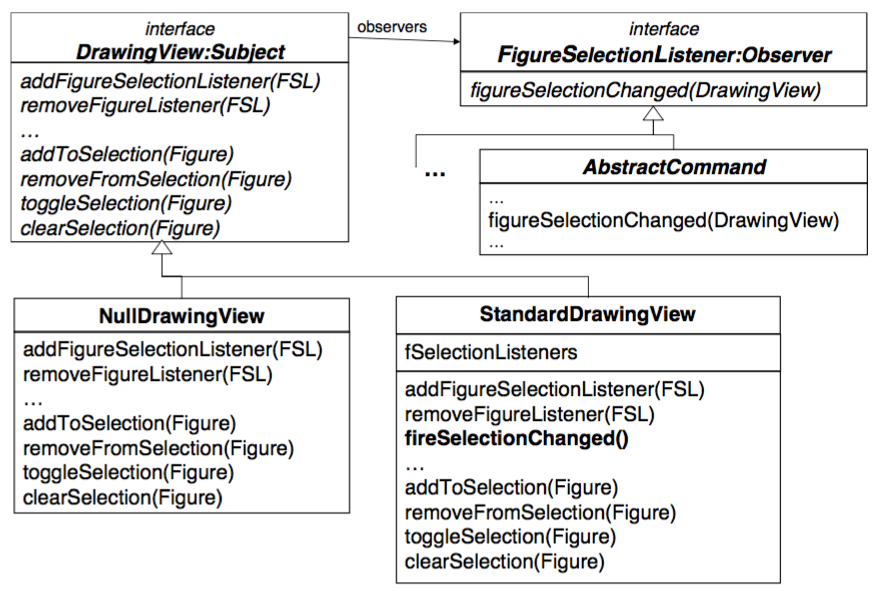
\includegraphics[width=.6\textwidth]{figures/BG_Observer_pattern_Selection_Listener.png}}
  	\caption{Observer pattern: Selection Listener \cite{marin2005approach}}
  	\label{fig:Selection_Listener}
\end{figure}

The \texttt{FigureSelectionListener} interface defines the \textit{Observer} role as its primary concern. 
The interface is implemented by all classes interested in changes of the selection of figures in a drawing view. 
The \texttt{DrawingView} interface partially defines the \textit{Subject} role. 
The \textit{Subject} role is a secondary concern for the \texttt{DrawingView} interface. 
Two classes implement this interface and only one, \texttt{StandardDrawingView}, contains a non-empty implementation of the \textit{Subject} role.

The aspect refactoring would be described as the aspect construct comprises both the \textit{Subject} and \textit{Observer} roles definition, and maintains a list of associations between each \textit{Subject} and its \textit{Observer} objects.
The type-based refactoring\cite{marin2005approach} distinguishes several crosscutting elements that occur in an implementation of the \textit{Observer} pattern: role superimposition, applied twice, for each of the two roles and consistent behavior to notify the observers of the changes in the subject object. 
The \texttt{GenericRole} (empty) interface documents the crosscutting type of role superimposition. 
Specific roles, like \textit{Observer} and \textit{Subject} (\texttt{SelectionSubject}) extend the interface.
These elements are shown in the figure \ref{fig:Concerns_Selection_Listener}.

\begin{figure}[h]
	\centering
  	\fbox{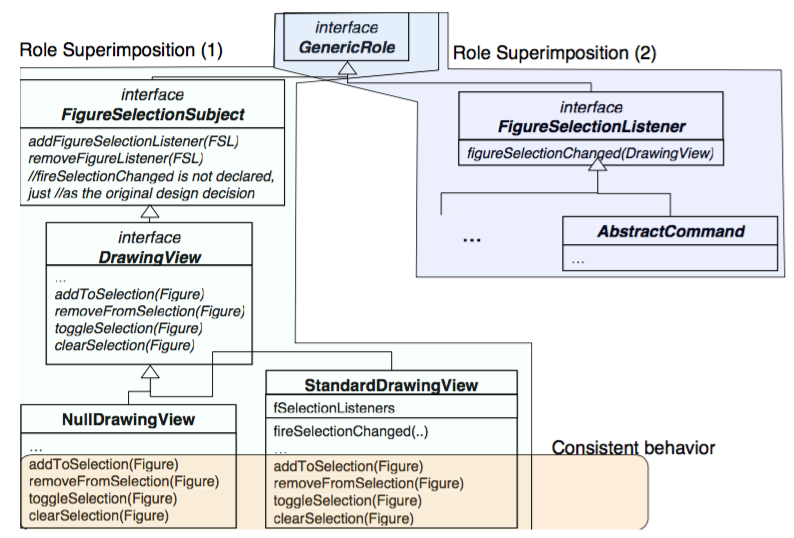
\includegraphics[width=.6\textwidth]{figures/BG_The_concern_types_in_Selection_Listener.png}}
  	\caption{The concern types in Selection Listener \cite{marin2005approach}}
  	\label{fig:Concerns_Selection_Listener}
\end{figure}

%%%%%%%%%%%%%%%%%%%%%%%%%%%%%%%%%%%%%%%%%%%%%%%%%%%%%%%%%%%%%%%%%%%%%%%%%%%%%%%
\subsubsection{Role-based Refactoring of \acrlong{ccc}}

%%%%%%%%%%%%%%%%%%%%%%%%%%%%%%%%%%%%%%%%%%%%%%%%%%%%%%%%%%%%%%%%%%%%%%%%%%%%%%%
\paragraph{Evaluation}

%%%%%%%%%%%%%%%%%%%%%%%%%%%%%%%%%%%%%%%%%%%%%%%%%%%%%%%%%%%%%%%%%%%%%%%%%%%%%%%
\subsection{The ``Undo'' Concern of JHotDraw}\label{The Undo Concern of JHotDraw}

%%%%%%%%%%%%%%%%%%%%%%%%%%%%%%%%%%%%%%%%%%%%%%%%%%%%%%%%%%%%%%%%%%%%%%%%%%%%%%%
\subsubsection{Evaluation}

%%%%%%%%%%%%%%%%%%%%%%%%%%%%%%%%%%%%%%%%%%%%%%%%%%%%%%%%%%%%%%%%%%%%%%%%%%%%%%%
\subsubsection{AspectJ Drawbacks in the Undo Solution}

%%%%%%%%%%%%%%%%%%%%%%%%%%%%%%%%%%%%%%%%%%%%%%%%%%%%%%%%%%%%%%%%%%%%%%%%%%%%%%%
% \subsection{The ``Persistence'' Concern of JHotDraw}

